\batchmode
\makeatletter
\def\input@path{{/Users/wesley/git/gwr/writeup/estimation//}}
\makeatother
\documentclass[english]{article}\usepackage[]{graphicx}\usepackage[]{color}
%% maxwidth is the original width if it is less than linewidth
%% otherwise use linewidth (to make sure the graphics do not exceed the margin)
\makeatletter
\def\maxwidth{ %
  \ifdim\Gin@nat@width>\linewidth
    \linewidth
  \else
    \Gin@nat@width
  \fi
}
\makeatother

\definecolor{fgcolor}{rgb}{0.345, 0.345, 0.345}
\newcommand{\hlnum}[1]{\textcolor[rgb]{0.686,0.059,0.569}{#1}}%
\newcommand{\hlstr}[1]{\textcolor[rgb]{0.192,0.494,0.8}{#1}}%
\newcommand{\hlcom}[1]{\textcolor[rgb]{0.678,0.584,0.686}{\textit{#1}}}%
\newcommand{\hlopt}[1]{\textcolor[rgb]{0,0,0}{#1}}%
\newcommand{\hlstd}[1]{\textcolor[rgb]{0.345,0.345,0.345}{#1}}%
\newcommand{\hlkwa}[1]{\textcolor[rgb]{0.161,0.373,0.58}{\textbf{#1}}}%
\newcommand{\hlkwb}[1]{\textcolor[rgb]{0.69,0.353,0.396}{#1}}%
\newcommand{\hlkwc}[1]{\textcolor[rgb]{0.333,0.667,0.333}{#1}}%
\newcommand{\hlkwd}[1]{\textcolor[rgb]{0.737,0.353,0.396}{\textbf{#1}}}%

\usepackage{framed}
\makeatletter
\newenvironment{kframe}{%
 \def\at@end@of@kframe{}%
 \ifinner\ifhmode%
  \def\at@end@of@kframe{\end{minipage}}%
  \begin{minipage}{\columnwidth}%
 \fi\fi%
 \def\FrameCommand##1{\hskip\@totalleftmargin \hskip-\fboxsep
 \colorbox{shadecolor}{##1}\hskip-\fboxsep
     % There is no \\@totalrightmargin, so:
     \hskip-\linewidth \hskip-\@totalleftmargin \hskip\columnwidth}%
 \MakeFramed {\advance\hsize-\width
   \@totalleftmargin\z@ \linewidth\hsize
   \@setminipage}}%
 {\par\unskip\endMakeFramed%
 \at@end@of@kframe}
\makeatother

\definecolor{shadecolor}{rgb}{.97, .97, .97}
\definecolor{messagecolor}{rgb}{0, 0, 0}
\definecolor{warningcolor}{rgb}{1, 0, 1}
\definecolor{errorcolor}{rgb}{1, 0, 0}
\newenvironment{knitrout}{}{} % an empty environment to be redefined in TeX

\usepackage{alltt}
\usepackage[T1]{fontenc}
\usepackage[latin9]{inputenc}
\setlength{\parskip}{\bigskipamount}
\setlength{\parindent}{0pt}
\usepackage{array}
\usepackage{bm}
\usepackage{multirow}
\usepackage{amsthm}
\usepackage{amsmath}
\usepackage{amssymb}
\usepackage{graphicx}
\usepackage{setspace}
\doublespacing

\makeatletter

%%%%%%%%%%%%%%%%%%%%%%%%%%%%%% LyX specific LaTeX commands.
%% Because html converters don't know tabularnewline
\providecommand{\tabularnewline}{\\}

%%%%%%%%%%%%%%%%%%%%%%%%%%%%%% Textclass specific LaTeX commands.
\usepackage[natbibapa]{apacite}
\theoremstyle{plain}
\newtheorem{thm}{\protect\theoremname}

\makeatother

\usepackage{babel}
\providecommand{\theoremname}{Theorem}
\IfFileExists{upquote.sty}{\usepackage{upquote}}{}
\begin{document}

\title{LAGR and its oracle properties}


\author{Wesley Brooks}

\maketitle

\section{Introduction}

Here goes the literature review. Essetial elements are:

- nonparametric regression

- varying coefficients regression

- adaptive lasso

- generalized linear models


\section{Varying coefficient models\label{sec:vcr}}


\subsection{Model}

Consider $n$ data points, observed at sampling locations $\bm{s}_{i}=(s_{i,1}\;\; s_{i,2})^{T}$
for $i=1,\dots,\bm{s}_{n}$, which are distributed in a spatial domain
$D\subset\mathbb{R}^{2}$ according to a density $f(\bm{s})$. For
$i=1,\dots,n$, let $y(\bm{s}_{i})$ and $\bm{x}(\bm{s}_{i})$ denote,
respectively, the univariate response and the $(p+1)$-variate vector
of covariates measured at location $\bm{s}_{i}$. At each location
$\bm{s}_{i}$, assume that the outcome is related to the covariates
by a linear model where the coefficients $\bm{\beta}(\bm{s}_{i})$
may be spatially-varying and $\varepsilon(\bm{s}_{i})$ is random
error at location $\bm{s}_{i}$. That is, 
\begin{align}
y(\bm{s}_{i})=\bm{x}(\bm{s}_{i})'\bm{\beta}(\bm{s}_{i})+\varepsilon(\bm{s}_{i}).\label{eq:lm(s)}
\end{align}


Further assume that the error term $\varepsilon(\bm{s}_{i})$ is normally
distributed with zero mean and variance $\sigma^{2}$, and that $\varepsilon(\bm{s}_{i})$,
$i=1,\dots,n$ are independent. That is, 
\begin{align}
\bm{\varepsilon}\overset{iid}{\sim}\mathcal{N}\left(0,\sigma^{2}\right).\label{eq:err}
\end{align}



\subsection{Augment the covariates and the coefficients with location interactions}

In the context of nonparametric regression, the boundary-effect bias
can be reduced by local polynomial modeling, usually in the form of
a locally linear model \cite{Fan-Gijbels-1996}. Here, locally linear
coefficients are estimated by augmenting the local design matrix with
covariate-by-location interactions in two dimensions as proposed by
\cite{Wang-2008b}. The augmented local design matrix at location
$\bm{s}_{i}$ is 
\begin{align}
\bm{Z}(\bm{s}_{i})=\left(\bm{X}\:\: L_{i}\bm{X}\:\: M_{i}\bm{X}\right)
\end{align}


where $\bm{X}$ is the unaugmented matrix of covariates, $L_{i}=\text{diag}\{s_{i'_{1}}-s_{i_{1}}\}$
and $M_{i}=\text{diag}\{s_{i'_{2}}-s_{i_{2}}\}$ for $i'=1,\dots,n$.

Now we have that $Y(\bm{s}_{i})=\left\{ \bm{Z}(\bm{s}_{i})\right\} _{i}^{T}\bm{\zeta}(\bm{s}_{i})+\varepsilon(\bm{s}_{i})$,
where $\left\{ \bm{Z}(\bm{s}_{i})\right\} _{i}^{T}$ is the $i$th
row of the matrix $\bm{Z}(\bm{s}_{i})$ as a row vector, and $\bm{\zeta}(\bm{s}_{i})$
is the vector of local coefficients at location $\bm{s}_{i}$, augmented
with the local gradients of the coefficient surfaces in the two spatial
dimensions, indicated by $\nabla_{u}$ and $\nabla_{v}$:

\[
\bm{\zeta}(\bm{s}_{i})=\left(\bm{\beta}(\bm{s}_{i})^{T}\;\;\nabla_{u}\bm{\beta}(\bm{s}_{i})^{T}\;\;\nabla_{v}\bm{\beta}(\bm{s}_{i})^{T}\right)^{T}
\]



\subsection{Local likelihood}

The total log-likelihood of the observed data is the sum of the log-likelihood
of each individual observation: 
\begin{align}
\ell\left\{ \bm{\zeta}\right\} =-(1/2)\sum_{i=1}^{n}\left[\log{\sigma^{2}}+\sigma^{-2}\left\{ y(\bm{s}_{i})-\bm{z}'(\bm{s}_{i})\bm{\zeta}(\bm{s}_{i})\right\} ^{2}\right].\label{eq:coefficients}
\end{align}


Since there are a total of $n\times3(p+1)+1$ parameters for $n$
observations, the model is not identifiable and it is not possible
to directly maximize the total likelihood. But since the coefficient
functions are smooth, the coefficients at location $\bm{s}$ can approximate
the coefficients within some neighborhood of $\bm{s}$, with the quality
of the approximation declining as the distance from $\bm{s}$ increases.

This intuition is formalized by the local likelihood, which is maximized
at location $\bm{s}$ to estimate the local coefficients $\bm{\zeta}(\bm{s})$:
\begin{align}
\mathcal{L}\left\{ \bm{\zeta}(\bm{s})\right\}  & =\prod_{i=1}^{n}\left\{ \left(2\pi\sigma^{2}\right)^{-1/2}\exp\left[-(1/2)\sigma^{-2}\left\{ y(\bm{s}_{i})-\bm{z}'(\bm{s}_{i})\bm{\zeta}(\bm{s})\right\} ^{2}\right]\right\} ^{K_{h}(\|\bm{s}-\bm{s}_{i}\|)},\label{eq:local-likelihood}
\end{align}


The weights are computed from a kernel function $K_{h}(\cdot)$ such
as the Epanechnikov kernel: 
\begin{align}
K_{h}(\|\bm{s}_{i}-\bm{s}_{i'}\|) & =h^{-2}K\left(h^{-1}\|\bm{s}_{i}-\bm{s}_{i'}\|\right)\notag\label{eq:epanechnikov}\\
K(x) & =\begin{cases}
(3/4)(1-x^{2}) & \mbox{ if }x<1,\\
0 & \mbox{ if }x\geq1.
\end{cases}
\end{align}


Thus, the local log-likelihood function is, up to an additive constant:
\begin{align}
\ell\left\{ \bm{\zeta}(\bm{s})\right\}  & =-(1/2)\sum_{i=1}^{n}K_{h}(\|\bm{s}-\bm{s}_{i}\|)\left[\log{\sigma^{2}}+\sigma^{-2}\left\{ y(\bm{s}_{i})-\bm{z}'(\bm{s}_{i})\bm{\zeta}(\bm{s})\right\} ^{2}\right].\label{eq:local-log-likelihood}
\end{align}



\subsection{Estimating the coefficients}

Letting $\bm{W}(\bm{s})$ be a diagonal weight matrix where $W_{ii}(\bm{s})=K_{h}(\|\bm{s}-\bm{s}_{i}\|)$,
the local likelihood is maximized by weighted least squares: 
\begin{align}
\mathcal{S}\left\{ \bm{\zeta}(\bm{s})\right\}  & =(1/2)\left\{ \bm{Y}-\bm{Z}(\bm{s})\bm{\zeta}(\bm{s})\right\} ^{T}\bm{W}(\bm{s})\left\{ \bm{Y}-\bm{Z}(\bm{s})\bm{\zeta}(\bm{s})\right\} ^{T}\notag\label{eq:zeta-hat}\\
\therefore\tilde{\bm{\zeta}}(\bm{s}) & =\left\{ \bm{Z}^{T}(\bm{s})\bm{W}(\bm{s})\bm{Z}(\bm{s})\right\} ^{-1}\bm{Z}^{T}(\bm{s})\bm{W}(\bm{s})\bm{Y}
\end{align}


Now Theorem 3 of \cite{Sun-Yan-Zhang-Lu-2014} says that, for any
given $\bm{{s}}$

\[
\sqrt{{nh^{2}f(\bm{{s}})}}\left[\hat{\bm{\beta}}(\bm{s})-\bm{\beta}(\bm{s})-(1/2)\kappa_{0}^{-1}\kappa_{2}h^{2}\left\{ \bm{\beta}_{uu}(\bm{s})+\bm{\beta}_{vv}(\bm{s})\right\} \right]\xrightarrow{{D}}N\left(\bm{0},\kappa_{0}^{-2}\nu_{0}\sigma^{2}\Psi^{-1}\right)
\]



\section{Local variable selection with LAGR\label{sec:lagr-gaussian}}

Estimating the local coefficients by (\ref{eq:zeta-hat}) relies on
\emph{a priori} variable selection. The goal of local adaptive grouped
regularization (LAGR) is to simultaneously select the locally relevant
predictors and estimate the local coefficients. The proposed LAGR
penalty is an adaptive $\ell_{1}$ penalty akin to the adaptive group
lasso \cite{Wang-Leng-2008,Zou-2006}.


\subsection{Variable groupings}

Each raw covariate in a LAGR model is grouped with its covariate-by-location
interactions. That is, $\bm{\zeta}_{j}(\bm{s})=\left(\beta_{j}(\bm{s})\;\;\;\nabla_{u}\beta_{j}(\bm{s})\;\;\;\nabla_{v}\beta_{j}(\bm{s})\right)^{T}$
for $j=1,\dots,p$. By the mechanism of the group lasso, variables
within the same group are included in or dropped from the model together.
The intercept group is left unpenalized.


\subsection{Write down the LAGR-penalized local likelihood}

The objective function for the LAGR at location $\bm{s}$ is the penalized
local sum of squares: 
\begin{align}
Q\{\bm{\zeta}(\bm{s})\} & =\mathcal{S}\left\{ \bm{\zeta}(\bm{s})\right\} +\mathcal{J}\{\bm{\zeta}(\bm{s})\}\notag\label{eq:adaptive-lasso-WLS}\\
 & =(1/2)\left\{ \bm{Y}-\bm{Z}(\bm{s})\bm{\zeta}(\bm{s})\right\} ^{T}\bm{W}(\bm{s})\left\{ \bm{Y}-\bm{Z}(\bm{s})\bm{\zeta}(\bm{s})\right\} ^{T}+\sum_{j=1}^{p}\phi_{j}(\bm{s})\|\bm{\zeta}_{j}(\bm{s})\|
\end{align}


which is the sum of the weighted sum of squares $\mathcal{S}\left\{ \bm{\zeta}(\bm{s})\right\} $
and the LAGR penalty $\mathcal{J}\{\bm{\zeta}(\bm{s})\}$.

The LAGR penalty for the $j$th group of coefficients $\bm{\zeta}_{j}(\bm{s})$
at location $\bm{s}$ is $\phi_{j}(\bm{s})=\lambda_{n}(\bm{s})\|\tilde{\bm{\zeta}}_{j}(\bm{s})\|^{-\gamma}$,
where $\lambda_{n}(\bm{s})>0$ is a the local tuning parameter applied
to all coefficients at location $\bm{s}$ and $\tilde{\bm{\zeta}}_{j}(\bm{s})$
is the vector of unpenalized local coefficients from (\ref{eq:zeta-hat}).


\subsection{Oracle properties of LAGR}
\begin{thm}[Asymptotic normality]
\label{theorem:normality} 



If $h^{-1}n^{-1/2}a_{n}\xrightarrow{p}0$ and $hn^{-1/2}b_{n}\xrightarrow{p}\infty$
then 
\[
h\sqrt{n}\left[\hat{\bm{\beta}}_{(a)}(\bm{s})-\bm{\beta}_{(a)}(\bm{s})-\frac{\kappa_{2}h^{2}}{2\kappa_{0}}\{\nabla_{uu}^{2}\bm{\beta}_{(a)}(\bm{s})+\nabla_{vv}^{2}\bm{\beta}_{(a)}(\bm{s})\}\right]\xrightarrow{d}N(0,f(\bm{s})^{-1}\kappa_{0}^{-2}\nu_{0}\sigma^{2}\Psi^{-1})
\]

\end{thm}

\begin{thm}[Selection consistency]
\label{theorem:selection}



If $h^{-1}n^{-1/2}a_{n}\xrightarrow{p}\infty$ and $hn^{-1/2}b_{n}\xrightarrow{p}\infty$
then $P\left\{ \|\hat{\bm{\zeta}}_{j}(\bm{s})\|=0\right\} \to0$ if
$j\le p_{0}$ and $P\left\{ \|\hat{\bm{\zeta}}_{j}(\bm{s})\|=0\right\} \to1$
if $j>p_{0}$. 
\end{thm}

\paragraph{Remarks}

Together, Theorem�\ref{theorem:normality} and Theorem \ref{theorem:selection}
indicate that the LAGR estimates have the same asymptotic distribution
as a local regression model where the nonzero coefficients are known
in advance \cite{Sun-Yan-Zhang-Lu-2014}, and that the LAGR estimates
of true zero coefficients go to zero with probability one. Thus, selection
and estimation by LAGR has the oracle property.


\paragraph{A note on rates}

To prove the oracle properties of LAGR, we assumed that $h^{-1}n^{-1/2}a_{n}\xrightarrow{p}0$
and $hn^{-1/2}b_{n}\xrightarrow{p}\infty$. Therefore, $h^{-1}n^{-1/2}\lambda_{n}(\bm{s})\to0$
for $j\le p_{0}$ and $hn^{-1/2}\lambda_{n}(\bm{s})\|\bm{\zeta}_{j}(\bm{s})\|^{-\gamma}\to\infty$
for $j>p_{0}$.

We require that $\lambda_{n}(\bm{s})$ can satisfy both assumptions.
Suppose $\lambda_{n}(\bm{s})=n^{\alpha}$, and recall that $h=O(n^{-1/6})$
and $\|\tilde{\bm{\zeta}}_{p}(\bm{s})\|=O(h^{-1}n^{-1/2})$. Then
$h^{-1}n^{-1/2}\lambda_{n}(\bm{s})=O(n^{-1/3+\alpha})$ and $hn^{-1/2}\lambda_{n}(\bm{s})\|\tilde{\bm{\zeta}}_{p}(\bm{s}\|^{-\gamma}=O(n^{-2/3+\alpha+\gamma/3})$.

So $(2-\gamma)/3<\alpha<1/3$, which can only be satisfied for $\gamma>1$.


\section{Extension to GLLMs\label{sec:lagr-gllm}}


\subsection{Model}

Generalized linear models (GLM) extend the linear model to distributions
other than gaussian. The generalized local linear model (GLLM) is
an extension of the GLM to varying coefficient models via local regression.

As was the case for local linear regression models, the GLLM coefficients
are smooth functions of location, called $\bm{\beta}(\bm{s})$. If
the response variable $y$ is from an exponential-family distribution
then its density is 

\[
f\left\{ y(\bm{s})|\bm{x}(\bm{s})\right\} =c\left\{ y(\bm{s})\right\} \times\exp\left[\frac{\theta(\bm{s})y(\bm{s})-b\left\{ \theta(\bm{s})\right\} }{a\left\{ \phi(\bm{s})\right\} }\right]
\]


where $\phi$ and $\theta$ are parameters and

\begin{align*}
E\left\{ y(\bm{s})|\bm{x}(\bm{s})\right\} = & \mu(\bm{s})=b'\left\{ \theta(\bm{s})\right\} \\
\theta(\bm{s})= & (g\circ b')^{-1}\left\{ \eta(\bm{s})\right\} \\
\eta(\bm{s})= & \bm{x}^{T}(\bm{s})\bm{\beta}(\bm{s})=g\left\{ \mu(\bm{s})\right\} \\
\text{\text{Var}}\left\{ y(\bm{s})|\bm{x}(\bm{s})\right\} = & b''\left\{ \theta(\bm{s})\right\} a\left\{ \phi(\bm{s})\right\} 
\end{align*}


The function $g(\cdot)$ is called the link function. If its inverse
$g^{-1}(\cdot)=b'(\cdot)$ then the composition $(g\circ b')(\cdot)$
is the identity function. This particular choice of $g$ is called
the canonical link. We follow the practice of \cite{Fan-Heckman-Wand-1995}
in assuming the use of the canonical link because it is simple and
because using an alternative link function would hardly affect the
local fit.

Under the canonical link function, the expressions for the mean and
variance of the response variable can be simplified to

\begin{align*}
E\left\{ y(\bm{s})|\bm{x}(\bm{s})\right\} = & g^{-1}\left\{ \eta(\bm{s})\right\} \\
\text{\text{Var}}\left\{ y(\bm{s})|\bm{x}(\bm{s})\right\} = & a\left\{ \phi(\bm{s})\right\} /g'\left\{ \mu(\bm{s})\right\} =V\left\{ \mu(\bm{s})\right\} \times a\left\{ \phi(\bm{s})\right\} 
\end{align*}
 


\subsection{Local quasi-likelihood}

Assuming the canonical link, all that is required is to specify the
mean-variance relationship via the variance function, $V\left\{ \mu(\bm{s})\right\} $.
Then the GLLM coefficients can be estimated by maximizing the local
quasi-likelihood 

\begin{align}
\ell\left\{ \bm{\zeta}(\bm{s})\right\}  & =\sum_{i=1}^{n}K_{h}(\|\bm{s}-\bm{s}_{i}\|)Q\left[g^{-1}\left\{ z'(\bm{s}_{i})\bm{\zeta}(\bm{s})\right\} ,Y(\bm{s}_{i})\right].
\end{align}


The local quasi-likelihood generalizes the local log-likelihood that
was used to estimate coefficients in the local linear model case.
The quasi-likelihood is convex, and is defined in terms of its derivative,
the quasi-score function

\[
\frac{\partial}{\partial\mu}Q(\mu,y)=\frac{y-\mu}{V(\mu)}.
\]



\subsection{Estimation}

Under these conditions, the local quasi-likelihood is maximized where

\begin{align}
\ell'\left\{ \hat{{\bm{\zeta}}}(\bm{s})\right\}  & =\sum_{i=1}^{n}K_{h}(\|\bm{s}-\bm{s}_{i}\|)\frac{y(\bm{s}_{i})-\hat{\mu}(\bm{s}_{i})}{V\left\{ \hat{\mu}(\bm{s}_{i})\right\} g'\left\{ \hat{\mu}(\bm{s}_{i})\right\} }\bm{z}(\bm{s}_{i})=\bm{0}_{3p}.
\end{align}


Except for the $K_{h}(\|\bm{s}-\bm{s}_{i}\|)$ term, this is the same
as the normal equations for estimating coefficients in a GLM. The
method of iteratively reweighted least squares (IRLS) is used to solve
for $\hat{{\bm{\zeta}}}(\bm{s})$.


\subsection{Distribution of the local coefficients}

The asymptotic distribution of the local coefficients in a varying-coefficients
GLM with a one-dimensional effect-modifying parameter are given in
\cite{Cai-Fan-Li-2000}. For coefficients that vary in two dimensions
(e.g. spatial location), the asymptotic distribution under the canonical
link is

\[
\sqrt{{nh^{2}f(\bm{{s}})}}\left[\hat{\bm{\beta}}(\bm{s})-\bm{\beta}(\bm{s})-(1/2)\kappa_{0}^{-1}\kappa_{2}h^{2}\left\{ \bm{\beta}_{uu}(\bm{s})+\bm{\beta}_{vv}(\bm{s})\right\} \right]\xrightarrow{{D}}N\left(\bm{0},\kappa_{0}^{-2}\nu_{0}V\left\{ \mu(\bm{s})\right\} \Psi^{-1}\right)
\]



\subsection{LAGR penalty}

As in the case of linear models, the LAGR for GLMs is a grouped $\ell_{1}$
regularization method. 


\subsection{Oracle properties of LAGR in the GLM setting}


\section{Simulations\label{sec:simulations}}

A simulation study was conducted to assess the performance of the
method described in Sections \ref{sec:vcr}--\ref{sec:lagr-gaussian}. 

Data were simulated on the domain $[0,1]^{2}$, which was divided
into a $30\times30$ grid. Each of $p=5$ covariates $X_{1},\dots,X_{5}$
was simulated by a Gaussian random field with mean zero and exponential
covariance function $\text{Cov}\left(X_{ji},X_{ji'}\right)=\sigma_{x}^{2}\exp{\left(-\tau_{x}^{-1}\delta_{ii'}\right)}$
where $\sigma_{x}^{2}=1$ is the variance, $\tau_{x}=0.1$ is the
range parameter, and $\delta_{ii'}$ is the Euclidean distance $\|\bm{s}_{i}-\bm{s}_{i'}\|_{2}$. 

Correlation was induced between the covariates by multiplying the
matrix $\bm{X}=\left(X_{1}\cdots X_{5}\right)$ by $\bm{R}$, where
$\bm{R}$ is the Cholesky decomposition of the covariance matrix $\bm{\Sigma}=\bm{R}'\bm{R}$.
The covariance matrix $\bm{\Sigma}$ is a $5\times5$ matrix that
has ones on the diagonal and $\rho$ for all off-diagonal entries,
where $\rho$ is the between-covariate correlation. 

The simulated response was $y_{i}=\bm{x}'_{i}\bm{\beta}_{i}+\varepsilon_{i}$
for $i=1,\dots,n$ where $n=900$ and the $\varepsilon_{i}$'s were
iid Gaussian with mean zero and variance $\sigma_{\varepsilon}^{2}$.
The simulated data included the response $y$ and five covariates
$x_{1},\dots,x_{5}$. The true data-generating model uses only $x_{1}$.
The variables $x_{2},\dots,x_{5}$ are included to assess performance
in model selection. 

Three different functions were used for the coefficient surface $\beta_{1}(\bm{s})$.
They are plotted in Figure \ref{fig:simulation-coefficient-functions},
and their mathematical forms are listed in (\ref{eq:simulation-coefficient-functions}).
The first is a step function, which is equal to zero in 40\% of the
spatial domain, equal to one in a different 40\% of the spatial domain,
and increases linearly in the middle 20\% of the domain. The second
is a gradient function, which increases linearly from zero at one
end of the domain to one at the other. The final coefficient function
is a parabola taking its maximum value of 1 at the center of the domain
and falling to zero at each corner of the domain. 

\begin{figure}
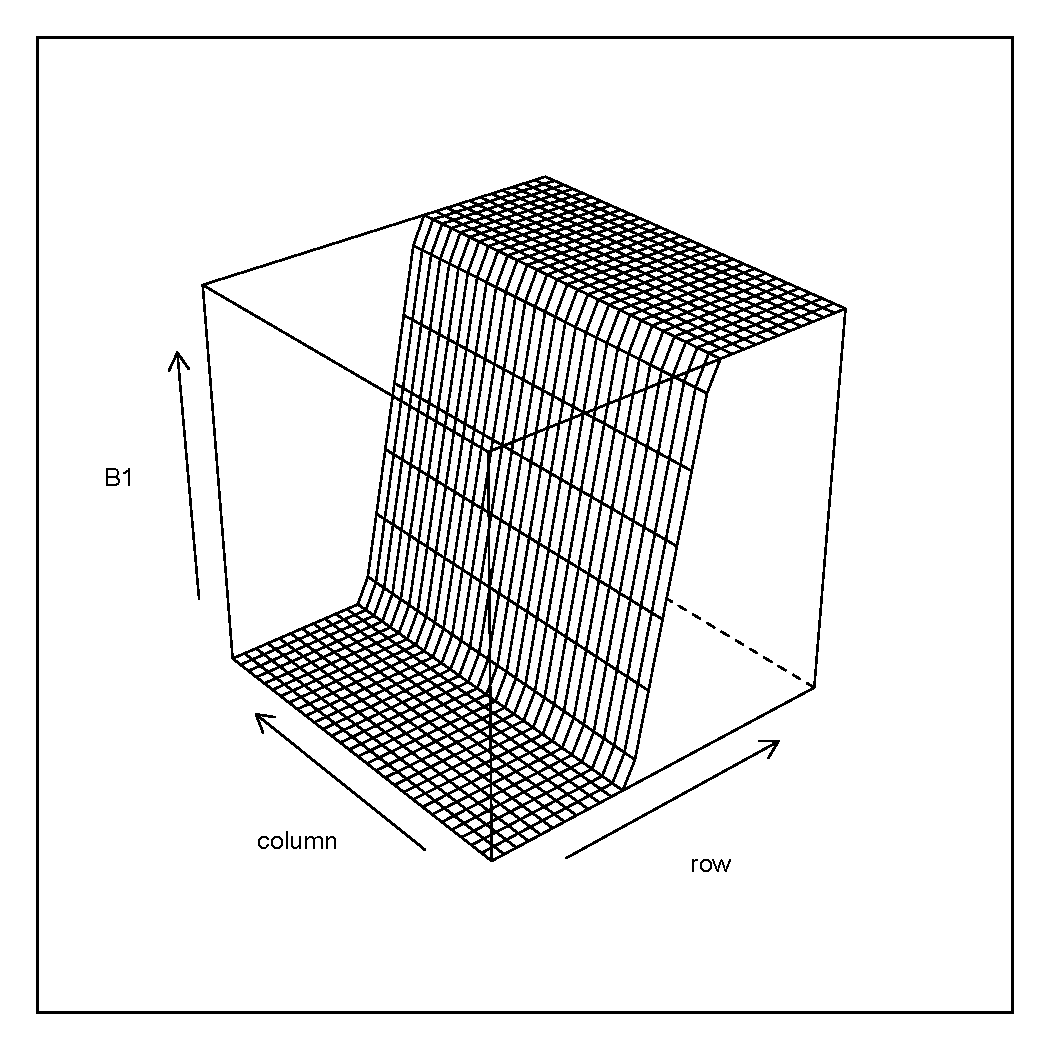
\includegraphics[width=0.33\textwidth]{0_Users_wesley_git_gwr_figures_simulation_step.pdf}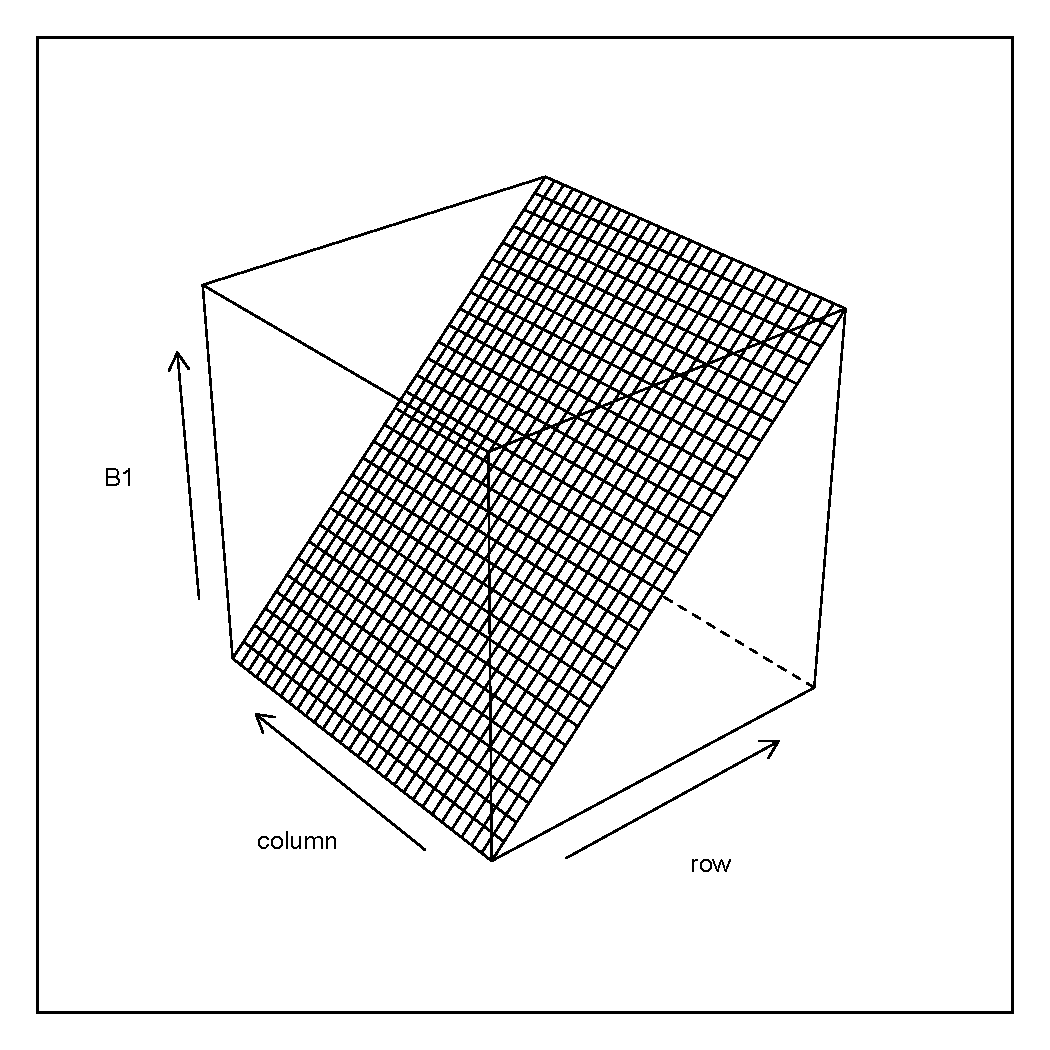
\includegraphics[width=0.33\textwidth]{1_Users_wesley_git_gwr_figures_simulation_gradient.pdf}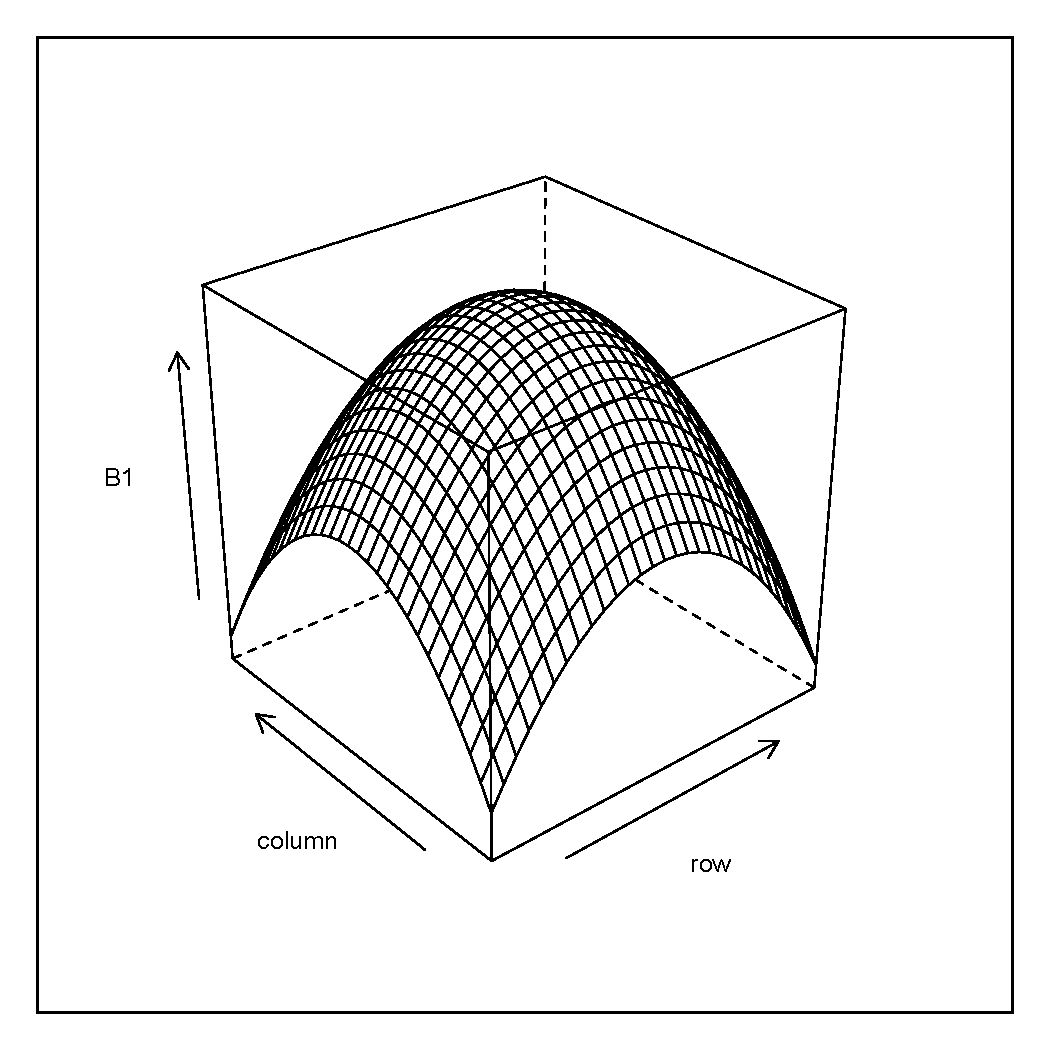
\includegraphics[width=0.33\textwidth]{2_Users_wesley_git_gwr_figures_simulation_parabola.pdf}

\protect\caption{These are, respectively, the step, gradient, and parabola functions
that were used for the coefficient function $\beta_{1}(\bm{s})$ in
the VCR model $y(\bm{s}_{i})=x_{1}(\bm{s}_{i})\beta_{1}(\bm{s}_{i})+\varepsilon(\bm{s}_{i})$
when generating the data for the simulation study.\label{fig:simulation-coefficient-functions}}
\end{figure}


\begin{align}
\beta_{step}(\bm{s})= & \ \ \begin{cases}
1 & if\ s_{x}>0.6\\
5s_{x}-2 & if\ 0.4<s_{x}\le0.6\\
0 & o.w.
\end{cases}\nonumber \\
\beta_{gradient}(\bm{s})= & \ \ s_{x}\nonumber \\
\beta_{parabola}(\bm{s})= & \ \ 1-\frac{(s_{x}-0.5)^{2}+(s_{y}-0.5)^{2}}{0.5}\label{eq:simulation-coefficient-functions}
\end{align}


In total, three parameters were varied to produce 18 settings, each
of which was simulated 100 times. There were three functional forms
for the coefficient surface $\beta_{1}(\bm{s})$; data was simulated
both with low ($\rho=0$), medium ($\rho=0.5$), and high ($\rho=0.9$)
correlation between the covariates; and simulations were made with
low ($\sigma_{\varepsilon}^{2}=0.25$) and high ($\sigma_{\varepsilon}^{2}=1$)
variance for the random error term. The simulation settings are enumerated
in Table \ref{tab:simulation-settings}. 

\begin{table}
\begin{tabular}{c|c|c}
$\beta_{1}(\bm{s})$ &
$\rho$ &
$\sigma_{\varepsilon}^{2}$\tabularnewline
\hline 
\multirow{6}{*}{step} &
\multirow{2}{*}{0} &
0.25\tabularnewline
\cline{3-3} 
 &  & 1\tabularnewline
\cline{2-3} 
 & \multirow{2}{*}{0.5} &
0.25\tabularnewline
\cline{3-3} 
 &  & 1\tabularnewline
\cline{2-3} 
 & \multirow{2}{*}{0.9} &
0.25\tabularnewline
\cline{3-3} 
 &  & 1\tabularnewline
\hline 
\multirow{6}{*}{gradient} &
\multirow{2}{*}{0} &
0.25\tabularnewline
\cline{3-3} 
 &  & 1\tabularnewline
\cline{2-3} 
 & \multirow{2}{*}{0.5} &
0.25\tabularnewline
\cline{3-3} 
 &  & 1\tabularnewline
\cline{2-3} 
 & \multirow{2}{*}{0.9} &
0.25\tabularnewline
\cline{3-3} 
 &  & 1\tabularnewline
\hline 
\multirow{6}{*}{parabola} &
\multirow{2}{*}{0} &
0.25\tabularnewline
\cline{3-3} 
 &  & 1\tabularnewline
\cline{2-3} 
 & \multirow{2}{*}{0.5} &
0.25\tabularnewline
\cline{3-3} 
 &  & 1\tabularnewline
\cline{2-3} 
 & \multirow{2}{*}{0.9} &
0.25\tabularnewline
\cline{3-3} 
 &  & 1\tabularnewline
\end{tabular}

\protect\caption{Listing of the simulation settings used to assess the performance
of LAGR models versus oracle selection and no selection.\label{tab:simulation-settings}}


\end{table}



\subsection{Methods for comparison}

The performance of LAGR was compared to that of a VCR model without
variable selection, and to a VCR model with oracular selection. Oracular
selection means that exactly the correct set of covariates was used
to fit each local model.


\subsection{Results}

The results are presented in terms of the mean integrated squared
error (MISE) of the coefficient surface estimates $\hat{\beta}_{1}(\bm{s}),\dots,\hat{\beta}_{5}(\bm{s})$,
the MISE of the fitted response $\hat{y}(\bm{s})$, and the frequency
with which the coefficient surface estimates $\hat{\beta}_{1}(\bm{s}),\dots,\hat{\beta}_{5}(\bm{s})$
in the LAGR model were zero.

The MISE of the estimates of $\beta_{1}(\bm{s})$ are in Table \ref{tab:x1-mise}.

% latex table generated in R 3.1.0 by xtable 1.7-3 package
% Wed Jun 25 23:47:37 2014
\begin{table}
\centering
\begin{tabular}{rrrr}
  & LAGR & none & oracle \\ 
  \hline
1 & \emph{0.02} & 0.02 & \textbf{0.01} \\ 
  2 & \emph{0.03} & 0.03 & \textbf{0.02} \\ 
  3 & \emph{0.02} & 0.02 & \textbf{0.01} \\ 
  4 & \emph{0.03} & 0.05 & \textbf{0.02} \\ 
  5 & \emph{0.03} & 0.05 & \textbf{0.01} \\ 
  6 & \emph{0.12} & 0.17 & \textbf{0.02} \\ 
  7 & 0.01 & \emph{0.01} & \textbf{0.00} \\ 
  8 & 0.03 & \emph{0.02} & \textbf{0.01} \\ 
  9 & 0.01 & \emph{0.01} & \textbf{0.00} \\ 
  10 & 0.04 & \emph{0.03} & \textbf{0.01} \\ 
  11 & \emph{0.03} & 0.04 & \textbf{0.00} \\ 
  12 & \emph{0.14} & 0.14 & \textbf{0.01} \\ 
  13 & 0.01 & \emph{0.01} & \textbf{0.01} \\ 
  14 & 0.03 & \emph{0.02} & \textbf{0.02} \\ 
  15 & 0.01 & \emph{0.01} & \textbf{0.01} \\ 
  16 & 0.03 & \emph{0.03} & \textbf{0.02} \\ 
  17 & \emph{0.02} & 0.04 & \textbf{0.01} \\ 
  18 & 0.17 & \emph{0.14} & \textbf{0.02} \\ 
  \end{tabular}
\caption{The MISE for the estimates of $\beta_1(\bm{s})$ in each simulation setting, under variable selection via LAGR, no variable selection, and oracular variable selection. Highlighting indicates the \textbf{lowest} and \emph{next-lowest} MISE.} 
\label{tab:x1-mise}
\end{table}


% latex table generated in R 3.1.0 by xtable 1.7-3 package
% Wed Jun 25 23:47:40 2014
\begin{table}
\centering
\begin{tabular}{rrrr}
  & LAGR & none & oracle \\ 
  \hline
1 & \emph{0.25} & 0.26 & \textbf{0.25} \\ 
  2 & \emph{1.00} & \textbf{1.00} & 0.99 \\ 
  3 & \emph{0.26} & 0.26 & \textbf{0.25} \\ 
  4 & \emph{0.99} & \textbf{1.00} & 0.98 \\ 
  5 & \emph{0.27} & 0.30 & \textbf{0.25} \\ 
  6 & \emph{1.08} & 1.14 & \textbf{0.98} \\ 
  7 & \emph{0.25} & \textbf{0.25} & 0.25 \\ 
  8 & \textbf{0.99} & \emph{0.99} & 0.97 \\ 
  9 & \emph{0.25} & \textbf{0.25} & 0.24 \\ 
  10 & \emph{1.00} & \textbf{1.00} & 0.97 \\ 
  11 & \emph{0.27} & 0.28 & \textbf{0.24} \\ 
  12 & \emph{1.09} & 1.12 & \textbf{0.97} \\ 
  13 & \emph{0.25} & \textbf{0.25} & 0.25 \\ 
  14 & \textbf{1.00} & \emph{1.00} & 0.98 \\ 
  15 & \textbf{0.25} & 0.25 & \emph{0.25} \\ 
  16 & \textbf{1.00} & \emph{1.00} & 0.97 \\ 
  17 & \emph{0.26} & 0.28 & \textbf{0.24} \\ 
  18 & 1.13 & \emph{1.12} & \textbf{0.98} \\ 
  \end{tabular}
\caption{The MISE for the fitted output in each simulation setting, under variable selection via LAGR, no variable selection, and oracular variable selection. Highlighting indicates the \textbf{closest} and \emph{next-closest} to the actual error variance $\sigma_\varepsilon^2$ for that setting.} 
\label{tab:misey}
\end{table}


% latex table generated in R 3.1.0 by xtable 1.7-3 package
% Wed Jun 25 23:47:42 2014
\begin{table}
\centering
\begin{tabular}{rr}
  & x \\ 
  \hline
1 & 0.97 \\ 
  2 & 0.96 \\ 
  3 & 0.96 \\ 
  4 & 0.92 \\ 
  5 & 0.86 \\ 
  6 & 0.85 \\ 
  7 & 0.96 \\ 
  8 & 0.95 \\ 
  9 & 0.94 \\ 
  10 & 0.92 \\ 
  11 & 0.80 \\ 
  12 & 0.85 \\ 
  13 & 0.97 \\ 
  14 & 0.94 \\ 
  15 & 0.95 \\ 
  16 & 0.88 \\ 
  17 & 0.79 \\ 
  18 & 0.78 \\ 
  \end{tabular}
\caption{Proportion of local models under each setting in which the coefficients $\beta_2(\bm{s}),\dots,\beta_5(\bm{s})$ are estimated as exactly zero.} 
\label{tab:pzero}
\end{table}



\section{Data example\label{sec:example}}

The proposed LAGR estimation method was used to estimate the coefficients
in a VCR model of the effect of some covariates on the price of homes
in Boston. The data source is the Boston house price data set of \cite{Harrison-Rubinfeld-1978,Gilley-Pace-1996,Pace-Gilley-1997},
which is based on the 1970 U.S. census. In the data, we have the median
price of homes sold in 506 census tracts (MEDV), along with some potential
predictor variables. The predictor variables are CRIM (the per-capita
crime rate in the tract), RM (the mean number of rooms for houses
sold in the tract), RAD (an index of how accessible the tract is from
Boston's radial roads), TAX (the property tax per \$10,000 of property
value), and LSTAT (the percentage of the tract's residents who are
considered ``lower status'').

The bandwidth parameter was set to 0.2 for a nearest neighbors-type
bandwidth, meaning that the sum of kernel weights for each local model
was 20\% of the total number of observations. The kernel used was
the Epanechnikov kernel.


\subsection{Results}

Estimates of the regression coefficients are plotted in Figure \ref{fig:boston-lagr-coefs}.

\begin{figure}

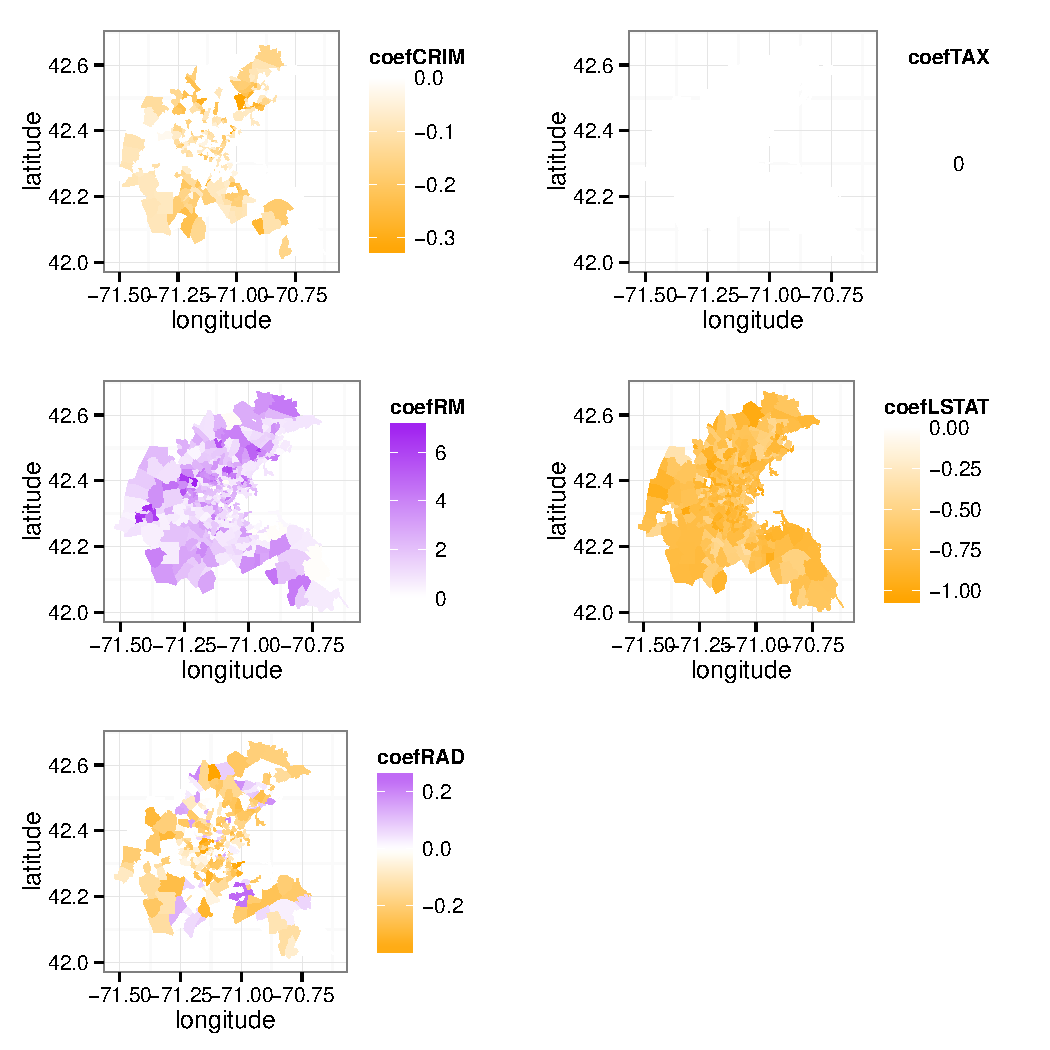
\includegraphics[width=\maxwidth]{figure/boston-plots} 


\caption{The coefficients for the boston house price data as estimated by LAGR.\label{fig:boston-lagr-coefs}}
\end{figure}

One interesting result is that the 

\appendix

\section{Proofs of theorems\label{app:proofs} }
\begin{proof}[Proof of theorem \ref{theorem:normality}]

\end{proof}
Define $V_{4}^{(n)}(\bm{u})$ to be the 
\begin{align}
\mkern-36muV_{4}^{(n)}(\bm{u}) & =Q\left\{ \bm{\zeta}(\bm{s})+h^{-1}n^{-1/2}\bm{u}\right\} -Q\left\{ \bm{\zeta}(\bm{s})\right\} \notag\label{eq:consistency}\\
 & \mkern-36mu=(1/2)\left[\bm{Y}-\bm{Z}(\bm{s})\left\{ \bm{\zeta}(\bm{s})+h^{-1}n^{-1/2}\bm{u}\right\} \right]^{T}\bm{W}(\bm{s})\left[\bm{Y}-\bm{Z}(\bm{s})\left\{ \bm{\zeta}(\bm{s})+h^{-1}n^{-1/2}\bm{u}\right\} \right]\notag\\
 & +\sum_{j=1}^{p}\phi_{j}(\bm{s})\|\bm{\zeta}_{j}(\bm{s})+h^{-1}n^{-1/2}\bm{u}_{j}\|\notag\\
 & -(1/2)\left\{ \bm{Y}-\bm{Z}(\bm{s})\bm{\zeta}(\bm{s})\right\} ^{T}\bm{W}(\bm{s})\left\{ \bm{Y}-\bm{Z}(\bm{s})\bm{\zeta}(\bm{s})\right\} -\sum_{j=1}^{p}\phi_{j}(\bm{s})\|\bm{\zeta}_{j}(\bm{s})\|\notag\\
 & \mkern-36mu=(1/2)\bm{u}^{T}\left\{ h^{-2}n^{-1}\bm{Z}^{T}(\bm{s})\bm{W}(\bm{s})\bm{Z}(\bm{s})\right\} \bm{u}-\bm{u}^{T}\left[h^{-1}n^{-1/2}\bm{Z}^{T}(\bm{s})\bm{W}(\bm{s})\left\{ \bm{Y}-\bm{Z}(\bm{s})\bm{\zeta}(\bm{s})\right\} \right]\notag\\
 & +\sum_{j=1}^{p}n^{-1/2}\phi_{j}(\bm{s})n^{1/2}\left\{ \|\bm{\zeta}_{j}(\bm{s})+h^{-1}n^{-1/2}\bm{u}_{j}\|-\|\bm{\zeta}_{j}(\bm{s})\|\right\} 
\end{align}


Note the different limiting behavior of the third term between the
cases $j\le p_{0}$ and $j>p_{0}$:


\paragraph{Case $j\le p_{0}$}

If $j\le p_{0}$ then $n^{-1/2}\phi_{j}(\bm{s})\to n^{-1/2}\lambda_{n}(\bm{s})\|\bm{\zeta}_{j}(\bm{s})\|^{-\gamma}$
and $|\sqrt{n}\left\{ \|\bm{\zeta}_{j}(\bm{s})+h^{-1}n^{-1/2}\bm{u}_{j}\|-\|\bm{\zeta}_{j}(\bm{s})\|\right\} |\le h^{-1}\|\bm{u}_{j}\|$
so 
\[
\lim\limits _{n\to\infty}\phi_{j}(\bm{s})\left(\|\bm{\zeta}_{j}(\bm{s})+h^{-1}n^{-1/2}\bm{u}_{j}\|-\|\bm{\zeta}_{j}(\bm{s})\|\right)\le h^{-1}n^{-1/2}\phi_{j}(\bm{s})\|\bm{u}_{j}\|\le h^{-1}n^{-1/2}a_{n}\|\bm{u}_{j}\|\to0
\]



\paragraph{Case $j>p_{0}$}

If $j>p_{0}$ then $\phi_{j}(\bm{s})\left(\|\bm{\zeta}_{j}(\bm{s})+h^{-1}n^{-1/2}\bm{u}_{j}\|-\|\bm{\zeta}_{j}(\bm{s})\|\right)=\phi_{j}(\bm{s})h^{-1}n^{-1/2}\|\bm{u}_{j}\|$.

And note that $h=O(n^{-1/6})$ so that if $hn^{-1/2}b_{n}\xrightarrow{p}\infty$
then $h^{-1}n^{-1/2}b_{n}\xrightarrow{p}\infty$.

Now, if $\|\bm{u}_{j}\|\ne0$ then 
\[
h^{-1}n^{-1/2}\phi_{j}(\bm{s})\|\bm{u}_{j}\|\ge h^{-1}n^{-1/2}b_{n}\|\bm{u}_{j}\|\to\infty
\]
. On the other hand, if $\|\bm{u}_{j}\|=0$ then $h^{-1}n^{-1/2}\phi_{j}(\bm{s})\|\bm{u}_{j}\|=0$.

Thus, the limit of $V_{4}^{(n)}(\bm{u})$ is the same as the limit
of $V_{4}^{*(n)}(\bm{u})$ where

\[
\mkern-72muV_{4}^{*(n)}(\bm{u})=\begin{cases}
(1/2)\bm{u}^{T}\left\{ h^{-2}n^{-1}\bm{Z}^{T}(\bm{s})\bm{W}(\bm{s})\bm{Z}(\bm{s})\right\} \bm{u}-\bm{u}^{T}\left[h^{-1}n^{-1/2}\bm{Z}^{T}(\bm{s})\bm{W}(\bm{s})\left\{ \bm{Y}-\bm{Z}(\bm{s})\bm{\zeta}(\bm{s})\right\} \right] & \mbox{ if }\|\bm{u}_{j}\|=0\;\forall j>p_{0}\\
\infty & \mbox{ otherwise }
\end{cases}.
\]


From which it is clear that $V_{4}^{*(n)}(\bm{u})$ is convex and
its unique minimizer is $\hat{\bm{u}}^{(n)}$:

\begin{align}
0 & =\left\{ h^{-2}n^{-1}\bm{Z}^{T}(\bm{s})\bm{W}(\bm{s})\bm{Z}(\bm{s})\right\} \hat{\bm{u}}^{(n)}-\left[h^{-1}n^{-1/2}\bm{Z}^{T}(\bm{s})\bm{W}(\bm{s})\left\{ \bm{Y}-\bm{Z}(\bm{s})\bm{\zeta}(\bm{s})\right\} \right]\notag\label{eq:limit}\\
\therefore\hat{\bm{u}}^{(n)} & =\left\{ n^{-1}\bm{Z}^{T}(\bm{s})\bm{W}(\bm{s})\bm{Z}(\bm{s})\right\} ^{-1}\left[hn^{-1/2}\bm{Z}^{T}(\bm{s})\bm{W}(\bm{s})\left\{ \bm{Y}-\bm{Z}(\bm{s})\bm{\zeta}(\bm{s})\right\} \right]\notag\\
\end{align}


By the epiconvergence results of \cite{Geyer-1994} and \cite{Knight-Fu-2000},
the minimizer of the limiting function is the limit of the minimizers
$\hat{\bm{u}}^{(n)}$. And since, by Lemma 2 of \cite{Sun-Yan-Zhang-Lu-2014},

\begin{equation}
\hat{\bm{u}}^{(n)}\xrightarrow{d}N\left(\frac{\kappa_{2}h^{2}}{2\kappa_{0}}\{\nabla_{uu}^{2}\bm{\zeta}_{j}(\bm{s})+\nabla_{vv}^{2}\bm{\zeta}_{j}(\bm{s})\},f(\bm{s})\kappa_{0}^{-2}\nu_{0}\sigma^{2}\Psi^{-1}\right)
\end{equation}
the result is proven.
\begin{proof}[Proof of theorem \ref{theorem:selection}]


We showed in Theorem \ref{theorem:normality} that $\hat{\bm{\zeta}}_{j}(\bm{s})\xrightarrow{p}\bm{\zeta}_{j}(\bm{s})+\frac{\kappa_{2}h^{2}}{2\kappa_{0}}\{\nabla_{uu}^{2}\bm{\zeta}_{j}(\bm{s})+\nabla_{vv}^{2}\bm{\zeta}_{j}(\bm{s})\}$,
so to complete the proof of selection consistency, it only remains
to show that $P\left\{ \hat{\bm{\zeta}}_{j}(\bm{s})=0\right\} \to1$
if $j>p_{0}$.
\end{proof}
The proof is by contradiction. Without loss of generality we consider
only the case $j=p$.

Assume $\|\hat{\bm{\zeta}}_{p}(\bm{s})\|\ne0$. Then $Q\left\{ \bm{\zeta}(\bm{s})\right\} $
is differentiable w.r.t. $\bm{\zeta}_{p}(\bm{s})$ and is minimized
where 
\begin{align}
0 & =\bm{Z}_{p}^{T}(\bm{s})\bm{W}(\bm{s})\left\{ \bm{Y}-\bm{Z}_{-p}(\bm{s})\hat{\bm{\zeta}}_{-p}(\bm{s})-\bm{Z}_{p}(\bm{s})\hat{\bm{\zeta}}_{p}(\bm{s})\right\} -\phi_{p}(\bm{s})\frac{\hat{\bm{\zeta}}_{p}(\bm{s})}{\|\hat{\bm{\zeta}}_{p}(\bm{s})\|}\notag\\
 & =\bm{Z}_{p}^{T}(\bm{s})\bm{W}(\bm{s})\left[\bm{Y}-\bm{Z}(\bm{s})\bm{\zeta}(\bm{s})-\frac{h^{2}\kappa_{2}}{2\kappa_{0}}\left\{ \nabla_{uu}^{2}\bm{\zeta}(\bm{s})+\nabla_{vv}^{2}\bm{\zeta}(\bm{s})\right\} \right]\notag\\
 & \mkern+72mu+\bm{Z}_{p}^{T}(\bm{s})\bm{W}(\bm{s})\bm{Z}_{-p}(\bm{s})\left[\bm{\zeta}_{-p}(\bm{s})+\frac{h^{2}\kappa_{2}}{2\kappa_{0}}\left\{ \nabla_{uu}^{2}\bm{\zeta}_{-p}(\bm{s})+\nabla_{vv}^{2}\bm{\zeta}_{-p}(\bm{s})\right\} -\hat{\bm{\zeta}}_{-p}(\bm{s})\right]\notag\\
 & \mkern+72mu+\bm{Z}_{p}^{T}(\bm{s})\bm{W}(\bm{s})\bm{Z}_{p}(\bm{s})\left[\bm{\zeta}_{p}(\bm{s})+\frac{h^{2}\kappa_{2}}{2\kappa_{0}}\left\{ \nabla_{uu}^{2}\bm{\zeta}_{p}(\bm{s})+\nabla_{vv}^{2}\bm{\zeta}_{p}(\bm{s})\right\} -\hat{\bm{\zeta}}_{p}(\bm{s})\right]\notag\\
 & \mkern+72mu-\phi_{p}(\bm{s})\frac{\hat{\bm{\zeta}}_{p}(\bm{s})}{\|\hat{\bm{\zeta}}_{p}(\bm{s})\|}\notag\\
\end{align}


So 
\begin{align}
\frac{h}{\sqrt{n}}\phi_{p}(\bm{s})\frac{\hat{\bm{\zeta}}_{p}(\bm{s})}{\|\hat{\bm{\zeta}}_{p}(\bm{s})\|} & =\bm{Z}_{p}^{T}(\bm{s})\bm{W}(\bm{s})\frac{h}{\sqrt{n}}\left[\bm{Y}-\bm{Z}(\bm{s})\bm{\zeta}(\bm{s})-\frac{h^{2}\kappa_{2}}{2\kappa_{0}}\left\{ \nabla_{uu}^{2}\bm{\zeta}(\bm{s})+\nabla_{vv}^{2}\bm{\zeta}(\bm{s})\right\} \right]\notag\label{eq:selection}\\
 & +\left\{ n^{-1}\bm{Z}_{p}^{T}(\bm{s})\bm{W}(\bm{s})\bm{Z}_{-p}(\bm{s})\right\} h\sqrt{n}\left[\bm{\zeta}_{-p}(\bm{s})+\frac{h^{2}\kappa_{2}}{2\kappa_{0}}\left\{ \nabla_{uu}^{2}\bm{\zeta}_{-p}(\bm{s})+\nabla_{vv}^{2}\bm{\zeta}_{-p}(\bm{s})\right\} -\hat{\bm{\zeta}}_{-p}(\bm{s})\right]\notag\\
 & +\left\{ n^{-1}\bm{Z}_{p}^{T}(\bm{s})\bm{W}(\bm{s})\bm{Z}_{p}(\bm{s})\right\} h\sqrt{n}\left[\bm{\zeta}_{p}(\bm{s})+\frac{h^{2}\kappa_{2}}{2\kappa_{0}}\left\{ \nabla_{uu}^{2}\bm{\zeta}_{p}(\bm{s})+\nabla_{vv}^{2}\bm{\zeta}_{p}(\bm{s})\right\} -\hat{\bm{\zeta}}_{p}(\bm{s})\right]
\end{align}


From Lemma 2 of \cite{Sun-Yan-Zhang-Lu-2014}, $\left\{ n^{-1}\bm{Z}_{p}^{T}(\bm{s})\bm{W}(\bm{s})\bm{Z}_{-p}(\bm{s})\right\} =O_{p}(1)$
and $\left\{ n^{-1}\bm{Z}_{p}^{T}(\bm{s})\bm{W}(\bm{s})\bm{Z}_{p}(\bm{s})\right\} =O_{p}(1)$.

From Theorem 3 of \cite{Sun-Yan-Zhang-Lu-2014}, we have that $h\sqrt{n}\left[\hat{\bm{\zeta}}_{-p}(\bm{s})-\bm{\zeta}_{-p}(\bm{s})-\frac{h^{2}\kappa_{2}}{2\kappa_{0}}\left\{ \nabla_{uu}^{2}\zeta_{-p}(\bm{s})+\nabla_{vv}^{2}\zeta_{-p}(\bm{s})\right\} \right]=O_{p}(1)$
and $h\sqrt{n}\left[\hat{\bm{\zeta}}_{p}(\bm{s})-\bm{\zeta}_{p}(\bm{s})-\frac{h^{2}\kappa_{2}}{2\kappa_{0}}\left\{ \nabla_{uu}^{2}\zeta_{p}(\bm{s})+\nabla_{vv}^{2}\zeta_{p}(\bm{s})\right\} \right]=O_{p}(1)$.

So the second and third terms of the sum in (\ref{eq:selection})
are $O_{p}(1)$.

We showed in the proof of \ref{theorem:normality} that $h\sqrt{n}\bm{Z}_{p}^{T}(\bm{s})\bm{W}(\bm{s})\left[\bm{Y}-\bm{Z}(\bm{s})\bm{\zeta}(\bm{s})-\frac{h^{2}\kappa_{2}}{2\kappa_{0}}\left\{ \nabla_{uu}^{2}\bm{\zeta}(\bm{s})+\nabla_{vv}^{2}\bm{\zeta}(\bm{s})\right\} \right]=O_{p}(1)$.

The three terms of the sum to the right of the equals sign in (\ref{eq:selection})
are $O_{p}(1)$, so for $\hat{\bm{\zeta}}_{p}(\bm{s})$ to be a solution,
we must have that $hn^{-1/2}\phi_{p}(\bm{s})\hat{\bm{\zeta}}_{p}(\bm{s})/\|\hat{\bm{\zeta}}_{p}(\bm{s})\|=O_{p}(1)$.

But since by assumption $\hat{\bm{\zeta}}_{p}(\bm{s})\ne0$, there
must be some $k\in\{1,\dots,3\}$ such that $|\hat{\zeta}_{p_{k}}(\bm{s})|=\max\{|\hat{\zeta}_{p_{k'}}(\bm{s})|:1\le k'\le3\}$.
And for this $k$, we have that $|\hat{\zeta}_{p_{k}}(\bm{s})|/\|\hat{\bm{\zeta}}_{p}(\bm{s})\|\ge1/\sqrt{3}>0$.

Now since $hn^{-1/2}b_{n}\to\infty$, we have that $hn^{-1/2}\phi_{p}(\bm{s})\hat{\bm{\zeta}}_{p}(\bm{s})/\|\hat{\bm{\zeta}}_{p}(\bm{s})\|\ge hb_{n}/\sqrt{3n}\to\infty$
and therefore the term to the left of the equals sign dominates the
sum to the right of the equals sign in (\ref{eq:selection}). So for
large enough $n$, $\hat{\bm{\zeta}}_{p}(\bm{s})\ne0$ cannot maximize
$Q$.

So $P\left\{ \hat{\bm{\zeta}}_{(b)}(\bm{s})=0\right\} \to1$. 

\bibliographystyle{chicago}
\bibliography{3_Users_wesley_git_gwr_references_gwr}

\end{document}
